\frametitle{Infrastructure}

\begin{minipage}{0.4\linewidth}
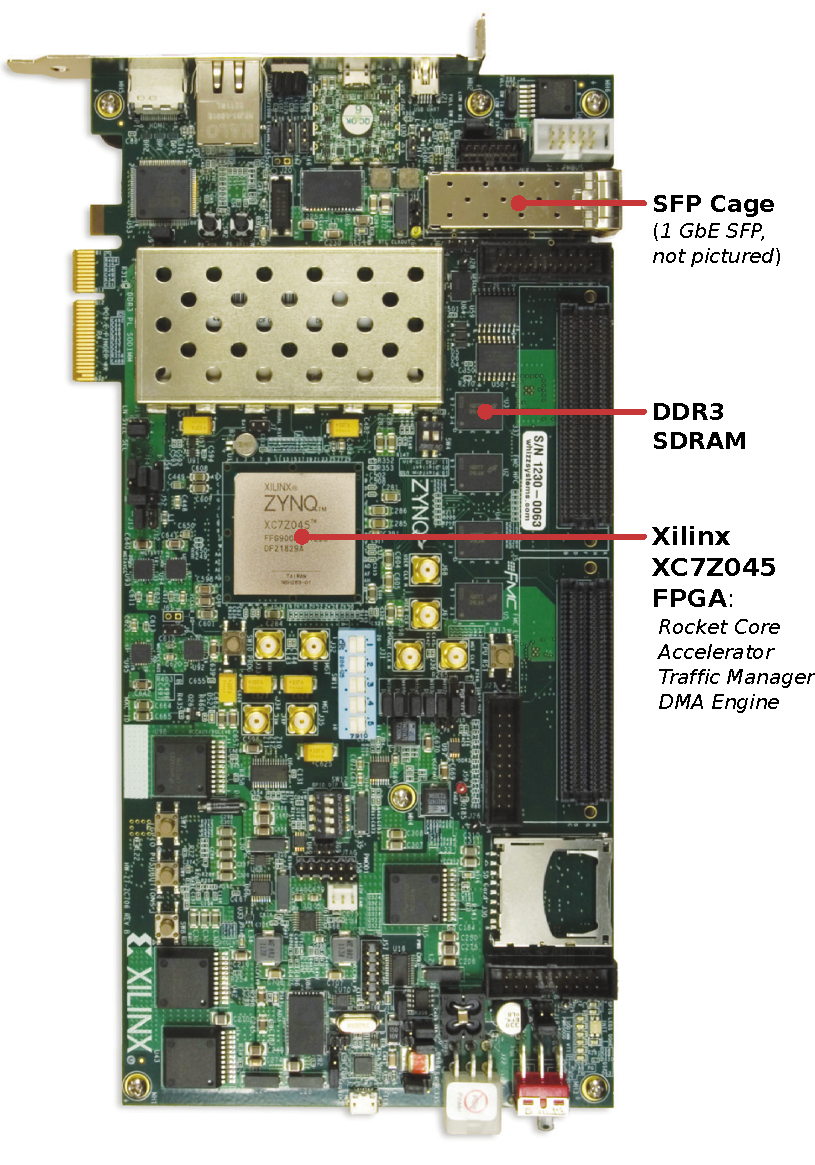
\includegraphics[width=\linewidth]{../img/zc706.pdf}
\end{minipage}
\hfill
\begin{minipage}{0.55\linewidth}
\alert{Xilinx ZC706 Evaluation Platform}
\begin{itemize}
\item ZYNQ-7000 SoC
\item Brocade 1GbE Copper SFP Transceiver
	\begin{itemize}
	\footnotesize
        \item Xilinx Tri-Mode Ethernet MAC
        \item Xilinx 1000Base-X PCS/PMA
	\end{itemize}
\item 64-bit RISC-V Rocket Core (\SI{50}{\mega\hertz})
	\begin{itemize}
	\footnotesize
	\item Single-issue, in-order, 6-stage pipeline
	\item ASIC version most nearly comparable with ARM Cortex-A5
	\end{itemize}
\end{itemize}
\vspace{\baselineskip}
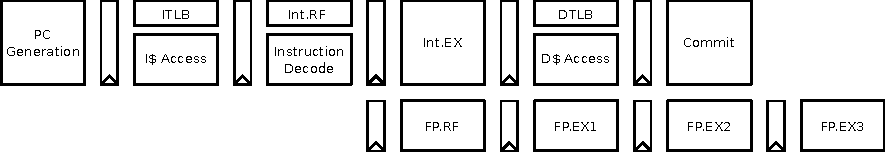
\includegraphics[width=\linewidth]{../img/rocket-pipeline.pdf}
\end{minipage}

\hrule
\vspace{0.5\baselineskip}
\begin{itemize}
\item No pre-existing I/O peripherals for the Rocket core
\item Built first RISC-V hardware device: register-mapped NIC
	\begin{itemize}
	\footnotesize
	\item Programmed I/O with custom Linux kernel driver
	\item First \texttt{telnet/ssh} session into a physical RISC-V machine
	\end{itemize}
\item Evolved to DMA-based NIC for performance
\end{itemize}
 



